\chapter{Background}\label{chap:background}\label{sec2}
% ---- TAKEAWAYS ----
% - A representation turns a molecule into a fixed-length vector of features. Each family captures different information and has its own weakness, so no single one captures everything.
% - Model families differ in how far one wrong label spreads: a tree keeps it in one leaf, an ensemble dilutes it, a neural network can memorise it.
% - Similarity only exists relative to a representation and a coefficient. Activity cliffs and uninformative features break the similar property principle.
% - Real label noise is not independent, identically distributed or Gaussian. It has heavy tails, shared offsets between laboratories and censoring at assay limits.
% - Learning with noisy labels (LNL) covers every method for training on wrong labels. Noise mitigation is the subset that changes the labels. No single method wins.
% - Every split in the thesis is group-aware, never random. NoiseInject supplies the noise and the robustness and uncertainty metrics used in later chapters.
% ---- END TAKEAWAYS ----

\section{Introduction}

% ---- NOTES: Introduction ----
% Takeaway: this chapter introduces, once, the ideas every later chapter refers back to.
% Paragraph 1: one-sentence roadmap, in section order.
% - Molecular representations: how a molecule becomes a fixed-length vector of features. Strings, fingerprints, descriptors, learned embeddings, graphs, and protein and antibody language-model embeddings.
% - Models: what each model family is, and why it might resist or absorb label noise.
% - Molecular similarity and activity cliffs: the assumption that similar molecules have similar properties.
% - Noise in molecular data: where label noise in real assay data comes from, and the seven artificial noise conditions.
% - Learning with noisy labels (LNL): training when some labels are wrong. Noise mitigation is the subset that removes, down-weights, smooths, relabels or corrects the labels.
% - NoiseInject: the open-source package that injects label noise and reports robustness and uncertainty metrics.
% - Evaluation: group-aware splitting, never random, and the predictive and uncertainty metrics.
% - Change: the sentence below names only two parts, and ends in a colon with no list after it.
% ---- END NOTES ----

I will now break down the two components of QSAR models: molecular representations and predictive models:


\section{Molecular Representations in QSAR}

% ---- NOTES: Molecular Representations in QSAR ----
% Takeaway: a representation maps a molecule to a fixed-length vector of features that a model takes as input.
% Takeaway: each family encodes different information and fails in a different way. This is what the hybrid in Chapter 5 builds on.
% Paragraph 1: what a representation is.
% - Definition 2.1, numbered: a molecular representation is a map from a molecule to a fixed-length numeric vector that a model takes as input.
% - Computing that vector is called featurization. Each position in the vector is one feature.
% - Features can be binary (a substructure present or absent), counts, real-valued descriptors, or the dimensions of a learned embedding.
% - The same definition covers the antibody inputs of Chapter 5: an amino-acid sequence mapped to a vector.
% - Change: the opening paragraph says "the type of input labels". The subject is the input features, not the labels.
% - Change: a numbered definition needs \usepackage{amsthm} and \newtheorem{definition}{Definition}[chapter] in the preamble.
% Paragraph 2: canonical and randomized one-hot SMILES.
% - One molecule has many valid SMILES strings. The canonical string is the single one a toolkit picks by fixed rules.
% - Randomized SMILES start the atom walk at a random atom, giving a different valid string each time \citep{ArusPous2019}.
% - Chapter 4's exploratory LNL study used both canonical and randomized one-hot SMILES.
% - Do not cite Bertoni2020 for one-hot SMILES. It is about bioactivity signatures inferred by neural networks, not SMILES encoding.
% Paragraph 3: MACCS and Avalon.
% - MACCS keys: a fixed list of 166 predefined substructure questions from MDL, re-examined for drug discovery by \citet{Durant2002}. As computed here it is 167 bits: the 166 keys plus one unused position.
% - Each MACCS bit answers one documented question, so its meaning is known without a lookup table. Substructures not on the list are not seen.
% - Change: cite Durant2002 for MACCS and rogers2010 for ECFP. The paragraph cites only Xie2020 for both.
% - Change: ECFP4 in this thesis ignores chirality (radius 2, 2,048 bits). The paragraph says "active chirality flags".
% - Avalon: a second hashed fingerprint, 2,048 bits here, built through RDKit \citep{Gedeck2006}. It shares ECFP's weakness: hashing folds different substructures onto one bit.
% - What Avalon hashes is not yet sourced. Check the Gedeck2006 full text before writing that sentence.
% Paragraph 4: mordred.
% - Mordred computes more than 1,800 two- and three-dimensional descriptors \citep{Moriwaki2018}. This thesis uses its 2D descriptors only, about 1,613 features.
% - Its weakness is the one already stated for descriptor vectors, at larger scale: multicollinearity. Chapter 4 shows that most features do not vary on a given dataset.
% Paragraph 5: MolFormer.
% - A transformer encoder trained on the SMILES strings of 1.1 billion unlabelled molecules from PubChem and ZINC \citep{ross2022}.
% - Linear attention and rotary position embeddings make training at that scale affordable \citep{ross2022}.
% - Used here as a fixed encoder: the vector is read out without fine-tuning.
% Paragraph 6: MHG-GNN, one or two sentences of its own.
% - Combines a molecular hypergraph grammar with a graph neural network \citep{kishimoto2023}.
% - Gives a fixed-length vector per molecule, like the SMILES language models, but read from the molecular graph.
% Paragraph 7 (new): protein and antibody language models, so Chapter 5 can point back.
% - Same idea as the chemical language models, applied to amino-acid sequences. A transformer trained self-supervised on residue sequences gives one vector per residue.
% - A vector per chain is usually the average of its residue vectors.
% - ESM-2 was scaled to 15 billion parameters, and atomic-level structure can be predicted from its representations \citep{Lin2023}.
% - ESM3 models sequence, structure and function together \citep{Hayes2025}.
% - ESM C: masked language models on protein sequences, metagenomic ones included, at 300 million, 600 million and 6 billion parameters \citep{Candido2026}. Preprint; say so.
% - SaProt adds one structure token per residue, from Foldseek, and was trained on about 40 million proteins \citep{Su2023SaProt}.
% - AntiBERTy was trained on 558 million natural antibody sequences \citep{Ruffolo2021AntiBERTy}.
% - AbLang-2 was trained on unpaired and paired chains to reduce the bias toward germline residues \citep{Olsen2024}.
% - IgT5 was trained on about 700 million unpaired sequences, then about 2 million paired heavy-light sequences, from the Observed Antibody Space \citep{Kenlay2024IgT5}. The "2 billion unpaired" figure belongs to IgBert, not IgT5.
% - Strength: dense vectors learned from far more sequences than any labelled dataset. Weakness: single features cannot be read, and computing them is costly.
% Closing: a comparison table.
% - Close the section with a table, one row per family: what it encodes, fixed or learned, typical length in features, whether a single feature can be read, main weakness.
% ---- END NOTES ----
The success of machine learning hinges on the quality of input data. Although the quality can refer to noise, which the majority of my work is centered around, in this case I'm talking about the type of input labels. Molecular representations provide different features with which QSAR models and noise detection techniques can be learned. However, a potential bottleneck on larger data sets should be noted; the more complex the data structure, the greater the computational cost. For smaller data sets, the number of parameters is limited by the size of the training set, to prevent overfitting. 

\begin{figure}[h]
	\centering 
	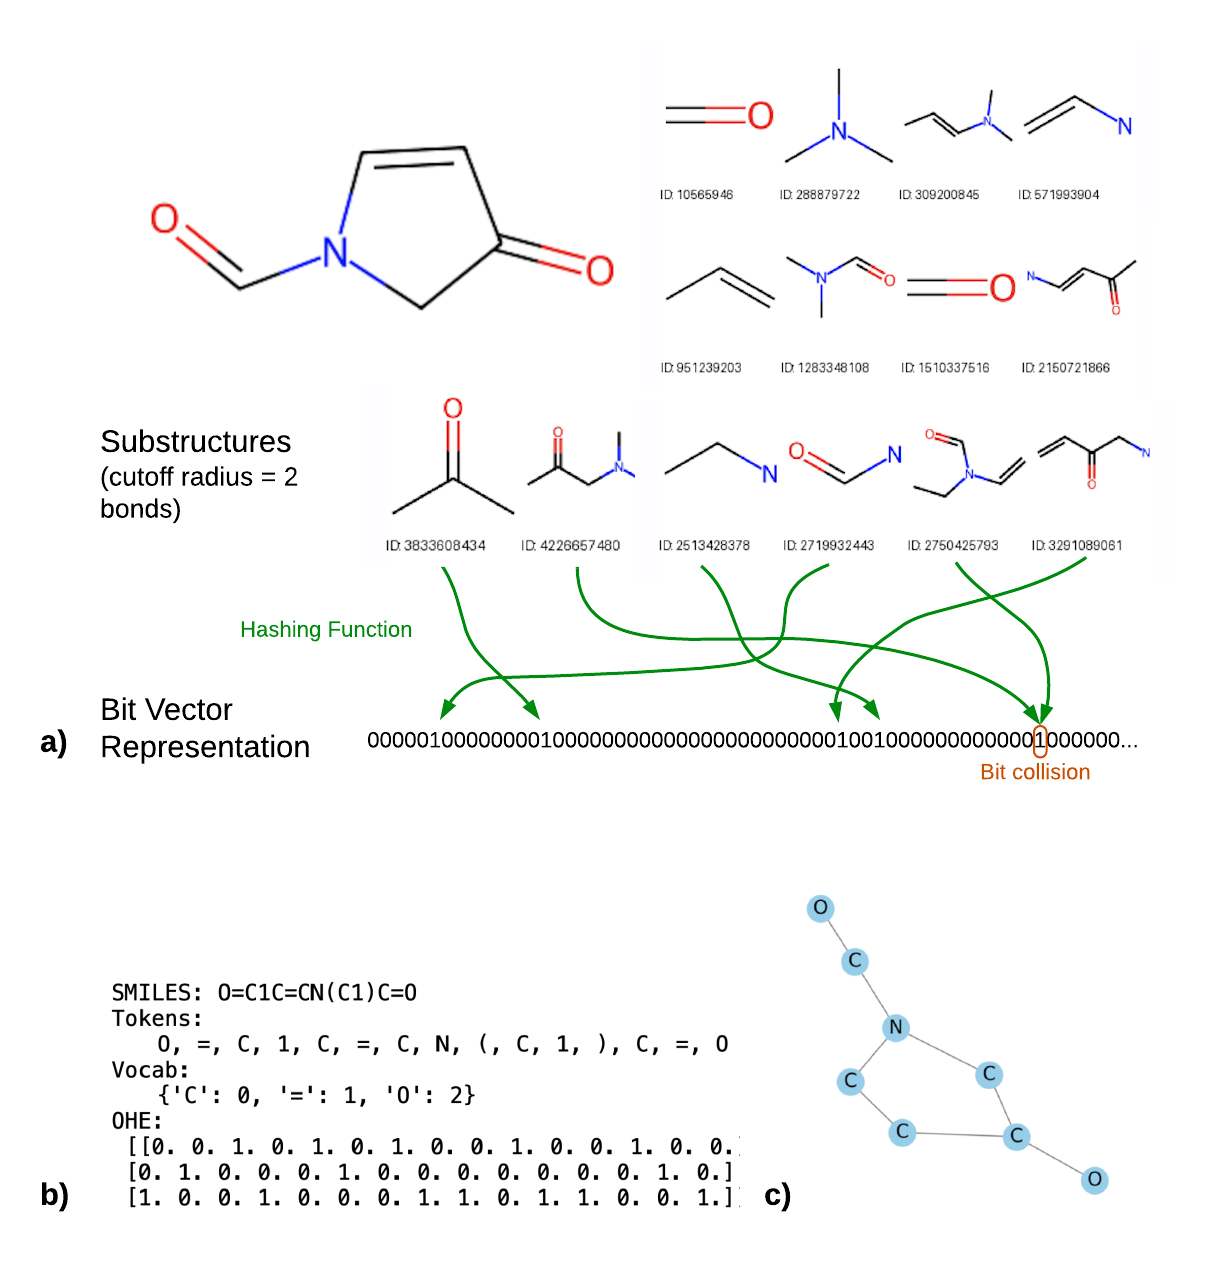
\includegraphics[width=1.05\textwidth]{molecular_representations.png}	
    \caption{\label{fig:molecular_representations}Visualisation of the molecule \lstinline{O=C1C=CN(C1)C=O} using three different methods: a) ECFP4 showing the molecule broken into substructures with circular neighbourhoods for each atom. Each substructure is hashed to produce unique identifiers, which are then compiled into a binary bit vector representing the presence or absence of specific substructures. b) SMILES tokenization and one-hot encoding of the molecule. The SMILES string is tokenized, and using a vocabulary of the most common tokens, these tokens are converted into a one-hot encoded matrix. c) Molecular graph representation where nodes represent atoms and edges represent bonds.}
\end{figure}

One of the most common and intuitive molecular representations are Simplified Molecular-Input Line-Entry System (SMILES) strings which consist of a sequence of ASCII characters generated by a fixed set of rules to specify a given chemical identity \citep{Weininger1988}. A common way to use SMILES strings as inputs to QSAR models is to tokenize and one-hot-encode them rather than to use the strings themselves \citep{TeachOpenCADD2023}. The strings are tokenized into atomic branches and symbols and mapped to indices of a vocabulary, and finally converted into binary vectors using one-hot encodings \citep{TeachOpenCADD2023}. This representation, referred to as one-hot-encoded SMILES, allows models to process molecular structures as bit-vector-based fingerprints or as sequences of vectors. Sequence-based models such as recurrent neural networks and transformers have proven to be particularly successful in capturing text semantics within a sequence. When applied to raw or one hot encoded (OHE) SMILES strings, these models can effectively capture the structure of the molecule in its textual representation \citep{TeachOpenCADD2023}. 

Another common representation is the molecular fingerprint, a vector containing information about the properties of the molecule in question. In a typical bit vector-based fingerprint, each bit accounts for the presence (1) or absence (0) of a given chemical feature or substructure \citep{Fassio2022}. One common fingerprint is the Molecular ACCess System (MACCS) key, a substructure key-based fingerprint that encodes predefined atom symbols and properties, as well as bond types \citep{Xie2020}. Another is the Extended Connectivity Fingerprint (ECFP), which encodes local neighborhoods around each atom and bond connectivity in molecules \citep{Xie2020}. ECFPs are typically constructed with a radius of 2, a length of 2048 bits, and active chirality flags. These existing molecular representations are well established and have been quite successful when coupled with QSAR models \citep{CortsCiriano2020, Sabando2021}. They are relatively simple, and as the bits can be mapped back to one or more substructures, they are human-interpretable, and furthermore easy-to-compute. However, they are subject to information loss due to bit collisions, which happens when two different substructures are encoded at the same bit position \citep{Fassio2022}. They are also based on a fixed procedure and are not trainable or adaptable to a particular dataset. Alternative representations that capture different structural, chemical, or physical features are able to overcome these limitations. 

Recent advances have led to the development of new molecular fingerprints. One such method is the Sort \& Slice (SNS) technique, an alternative to hash-based folding for pooling ECFP substructures \citep{sns}. Sort \& Slice begins by sorting all circular substructures in the training set according to their frequency of occurrence. It then "slices" away all but the $N$ most frequent substructures, which are subsequently used to generate an $N$-dimensional, bit-collision-free binary fingerprint. This approach solves the ambiguity problem of hashed fingerprints, where multiple substructures might be encoded at the same bit position, making it very interpretable \citep{sns}. Sort \& Slice fingerprints outperform ECFP4 with standard hash-based folding methods across various molecular property prediction tasks. These experiments consisted of different data splitting techniques, machine learning models, fingerprint diameters, fingerprint dimensions, and atomic invariants \citep{sns}. Furthermore, Sort \& Slice outperformed advanced substructure selection schemes such as filtered fingerprints and mutual information maximization \citep{sns}. 


Neural fingerprints are a category of learned  representations that overcome the fixed, hard-coded nature of traditional fingerprints. Unlike ECFP or MACCS keys, which rely on predefined hashing schemes or substructure catalogues, neural fingerprints train on molecular data to capture chemical information \citep{Jaeger2018, Chithrananda2020}. These representations are the result of deep learning architectures that have learned dense, continuous embeddings which can be used for downstream tasks. 

% TODO: review, needs manual review
Mol2vec, which adapts the Word2vec algorithm from NLP to molecular substructures \citep{Jaeger2018}, is common neural fingerprint. Mol2vec treats molecules like "sentences" and circular substructures derived from Morgan fingerprints like "words". The model learns vector embeddings for each substructure through unsupervised training, such that chemically similar substructures are mapped to nearby points in the embedding space \citep{Jaeger2018}. The embeddings of all present substructures are summed to obtain a full representation. This approach produces 300-dimensional dense vectors \citep{Jaeger2018}. Mol2vec has performed strongly on various QSAR benchmarks, matching or exceeding Morgan fingerprints on solubility and bioactivity prediction tasks \citep{Jaeger2018}.

Transformer-based architectures have also been applied to molecular representation learning, similarly stemming from NLPs ideas. MolBERT applies a bidirectional transformer to learn molecular representations from SMILES strings through self-supervised pre-training \citep{Fabian2020}. The model has domain-relevant auxiliary adaptations, such as the prediction of calculated physicochemical properties alongside the masked token prediction, to improve the chemical fidelity of the learned embeddings \citep{Fabian2020}. MolBERT demonstrated improvements over traditional fingerprints and graph-based methods on Virtual Screening and QSAR benchmarks \citep{Fabian2020}. ChemBERTa is another transformer-based approach which pre-trains masked language models on SMILES data from PubChem \citep{Chithrananda2020}.  ChemBERTa uses a tokenization strategy adapted for the SMILES notation, which allows the model to learn representations of atoms and functional groups through self-supervised learning \citep{Chithrananda2020}. Attention visualization reveals that ChemBERTa learns chemically meaningful patterns, with different attention heads specializing in functional groups, ring structures, or SMILES syntax \citep{Chithrananda2020}. ChemBERTa-2, an optimized variant pre-trained in 77 million compounds, achieved even stronger performance than the original ChemBERTa in MoleculeNet benchmarks \citep{Ahmad2022}.

Neural fingerprints provide several advantages over traditional fingerprints. They produce dense continuous vectors that avoid sparseness and information loss from bit collisions \citep{Jaeger2018}. They can also be pre-trained once on large unlabeled datasets and then fine-tuned for specific downstream tasks, opening the door to transfer learning \citep{Chithrananda2020, Fabian2020}. However, these methods are often computationally expensive \citep{Jaeger2018} and due to their black-box nature, they are not as interpretable.  \citep{Chithrananda2020}. However, attention mechanisms can have some degree of interpretability through visualization \citep{Chithrananda2020}.

Beyond fingerprints, physicochemical-descriptor vectors (PDVs) are a class of continuous-value molecular descriptors that encode structural and chemical properties of molecules \citep{Todeschini2009}. Unlike binary fingerprints or graph-based representations, PDVs aggregate atom and bond-level quantities into fixed-length feature vectors that capture a wide variety of information about a molecule and its structure \citep{Mauri2006}. PDVs typically consist of hundreds of properties including constitutional descriptors such as molecular weight, atom and bond counts, and heteroatom ratios; topological indices encoding molecular connectivity patterns; physicochemical properties such as logP (lipophilicity), molar refractivity, and topological polar surface area; and electronic descriptors derived from partial charges and polarizabilities \citep{Todeschini2009, Cherkasov2014}. The \texttt{RDKit} cheminformatics toolkit provides a comprehensive suite of more than 200 molecular descriptors that cover these categories \citep{rdkit}. PDVs are very interpretable; each descriptor has a clear physicochemical meaning \citep{Cherkasov2014}. They are also less computationally expensive than some 3D methods or neural fingerprints, with many descriptors simply requiring a 2D molecular structure without conformer generation or extensive pre-training. This efficiency makes PDVs particularly appropriate for high-throughput applications. However, it is also possible to use descriptors based on 3D components \citep{Mauri2006}.

However, PDVs have limitations. The dimensionality of PDV feature spaces can lead to problems with multicollinearity \citep{Todeschini2009}. This can be mitigated by feature selection or dimensionality reduction techniques \citep{Cherkasov2014}. Additionally, PDVs encode molecular properties as aggregated global features, which may not capture fine-grained structural details such as specific substructure arrangements or local chemical environments, information important for particular endpoints \citep{Mauri2006}.

One of the more intuitive representations are molecular graphs. These graphs can be categorized into 2D and 3D graphs. 2D graphs rely on adjacency matrices that encode topological atom- and bond-level features but leave out geometric properties such as bond angles or torsion, meaning they may fail to capture stereochemistry. 3D graphs incorporate these spatial features, but are often limited by remaining in a single conformation \citep{Zhichun2023}. A standard 3D molecular graph is constructed such that each molecule is represented as $G = (V,E)$ with node features $\mathbf{x}_i$ and edge features $\mathbf{e}_{ij}$. Nodes encode atom type, degree, hybridization, aromaticity, and formal charge; edges encode bond order and conjugation \citep{Zhichun2023}. 

% TODO: review, needs manual review
Another common molecular graph is the standard distance compatibility molecular graph, in which atoms and bonds are mapped to sets of nodes and edges \citep{David2020, Hnig2022}. These molecular graphs are typically 2D objects that represent 3D information such as atomic coordinate, bond angles, chirality, etc. \citep{David2020}. However, there are alternative molecular graph representations such as graphs with quantum 3D embeddings, weight alignment graphs, association graphs containing pairs of molecules, and geometric interaction graph neural network that incorporate 3D structures and physical interactions \citep{Hnig2022, yan2023, Yang2023GIGN}. \cite{Du2022} developed hybrid 2D and 3D graphs, combining 3D data, guaranteeing precision and completeness by providing unabridged information, and 2D data, providing chemical intuitions for guidance, in a zipper-like arrangement. These graphs pose various challenges, such as the atoms being localized at voxels creating issues with the points being too sparse, leading to poor performance. \cite{Kuzminykh2018} developed a novel approach in which atoms are extended to fill nearby voxels with a wave transformation.
      
These graph representations do not highlight specific substructures or specific arrangements of atoms and bonds within each molecule. The substructures contain functional groups that are related to a range of chemical properties and are potentially involved in downstream tasks related to the function of molecules. \cite{Bouritsas2023} developed graph substructure networks, a topologically aware message passing scheme based on substructure encoding. The method involves encoding structural roles based on the appearance of specific substructures and using them in message passing updates. Since message-passing GNNs are at most as powerful as the Weissfeiler Leman test, they cannot isolate sufficient features from the graph structure \citep{Bouritsas2023}. Graph substructure networks, on the other hand, capture these substructure-related features. And recent research has highlighted the abilities of pretrained GNN encoders produce embeddings on unlabeled datasets that capture structural features \citep{kishimoto2023, ross2022}. 

% TODO: review, needs manual review
\cite{Kolmar2021} examined the predictive limits of QSAR in the presence of noise, showing that by learning the underlying trends rather than fitting to noise, the models can achieve predictions more accurate than those of their training data. They assumed experimental noise could be modeled as Gaussian-distributed, using the Central Limit Theorem to argue that aggregated experimental measurements from multiple independent error sources exhibit a Gaussian distribution. However, \cite{Heid2023} used mean-variance estimation and bias-variance decomposition to show that noise can be tied to specific modalities, for example structure dependence. As an example, nitrogen-containing functional groups introduce measurement deviations, implying the presence of systematic noise. 

\section{Models for molecular property prediction}
% ---- NOTES: Models for molecular property prediction ----
% Takeaway: model families differ in how far one wrong label spreads. A tree keeps it in one leaf, an ensemble dilutes it, a network can memorise it.
% Paragraph 1: models treat labels as true values.
% - Models treat each label as an exact value, not a draw from a distribution. So they can fit the noise and report scores that are too optimistic.
% - The evidence (too few repeat measurements per molecule, Kolmar2021) is in the Chapter 1 introduction. Point there.
% Paragraphs 2-4: decision trees.
% - A tree splits the feature space by if-then rules; each leaf predicts from the training molecules that land in it \citep{Breiman1984}.
% - Non-linear, no distributional assumptions \citep{Breiman1984, Svetnik2003}.
% - A noisy label only affects predictions for molecules in its own leaf.
% Paragraph 5: ensembles of trees.
% - Random forests: bootstrap samples plus a random subset of features at each split \citep{Breiman2001}.
% - Gradient boosting: each tree fits the residuals of the trees before it \citep{Chen2016}.
% - Bootstrapping and averaging dilute any one noisy label.
% Paragraphs 6-7: feed-forward neural networks.
% - Training moves the weights to reduce the gap between prediction and label, by backpropagation \citep{Rumelhart1986}.
% - The usual QSAR network is a fully connected feed-forward network on fingerprints or descriptors \citep{Ma2015}.
% - Change: backpropagation is cited to Hornik1989, which proves universal approximation. Cite Rumelhart1986.
% - Change: "it's layers" should be "its layers".
% - Change: wu2018 does not state the "2-3 hidden layers with 128-512 units" recommendation.
% Paragraph 8: why networks struggle on QSAR data and under label noise.
% - Trees and tree ensembles often beat networks on small datasets and overfit less \citep{Baskin2008, Koutsoukas2017}.
% - Change: "don't rely on a static 3D molecular structure like NNs do" is wrong for the networks in this thesis. They take fixed-length vectors, never 3D coordinates.
% - Networks can fit randomly assigned labels perfectly \citep{Zhang2017}. So they can also fit noisy labels.
% - Change: the last sentence cites Zhang2017 for robust losses, mixup and label smoothing. Cite robust losses \citep{Ghosh2017}, mixup \citep{Zhang2018mixup}, label smoothing \citep{Szegedy2015}. Northcutt2021 for confident learning is correct.
% - These are all LNL methods. Label smoothing and removing examples flagged by confident learning change the labels, so they are noise mitigation. Robust losses and mixup change training instead.
% Paragraph 9: graph neural networks.
% - All models above take a fixed-length vector. Graph networks take the molecular graph.
% - GCN: each atom's vector is updated from a normalised, weighted sum of its neighbours' vectors \citep{Kipf2017}.
% - GIN: a plain sum followed by a trainable MLP; as powerful as the Weisfeiler-Lehman test at telling graphs apart \citep{Xu2019}.
% - Change: add Kipf2017 for GCNs. "Convolutional Networks (GCNs)" is missing "Graph". Write "activity cliffs" in lower case.
% - No graph network is trained as a predictor in this thesis. MHG-GNN, a GIN-based autoencoder, is used only as a fixed-length embedding \citep{kishimoto2023}.
% Paragraph 10: which chapters use which families, one sentence.
% - Chapter 3: tree ensembles, SVMs, Gaussian processes and feed-forward networks, including probabilistic versions. Chapters 5 and 6: tree ensembles, an SVM and a feed-forward network, plus a Gaussian process on datasets under 1,000 molecules.
% ---- END NOTES ----

One key issue with QSAR models is the standard assumption that labels represent true values. Most ML models rely on the assumption that the training data is, in fact, an accurate reflection of the population. Therefore, they treat these potentially noisy labels as discrete quantities rather than distributions, which opens the door to overfitting to noise and giving unduly optimistic assessments of the models.

There are a wide variety of model architectures that can be used for QSAR modeling. Starting off with simpler and more explainable models, we have tree-based methods. Decision trees are non-parametric supervised learning algorithms that perform recursive binary partitioning of the feature space \citep{Breiman1984}. A decision tree builds a predictive model by learning a series of if-then rules that recursively split the data based on given feature values, creating a tree  where internal nodes represent decision rules, branches represent the results of those decisions, and leaf nodes contain predicted values or class labels \citep{Breiman1984}. Each recursive split is chosen to maximize  homogeneity within the resulting partitions. For classification, Gini impurity is commonly used and for regression, mean squared error reduction \citep{Breiman1984}.

There are several properties that make decision trees a good foundation for QSAR modeling. First, they handle non-linear relationships between molecular descriptors and target properties without requiring explicit feature engineering or transformation \citep{Breiman1984}. They also do not make assumptions about the underlying distribution of the data, making them robust to violations of parametric assumptions that can limit linear regression or other classical methods \citep{Svetnik2003}. 

Decision trees handle data in a "contributory" rather than "consensus" manner. In consensus methods such as linear regression or neural networks, every data point influences the prediction at every other point in the feature space. Tree-based methods make predictions based on the subset of training samples that fall into the same leaf node as the test point \citep{Breiman1984}. This mechanism essentially quarantines outliers in their respective leaf nodes, limiting their impact on predictions for samples in other regions or chemical domains. 

Individual decision trees tend to have high variance and often overfit, particularly at large depths \citep{Breiman1984}. Small modifications made to the training data can result in large differences in the structure of the tree, resulting in unstable predictions \citep{Breiman2001}. Ensemble methods are used to counteract this instability, aggregating predictions from many trees. Random forests (RFs) aggregate predictions from trees trained on bootstrap samples of data with random subsets of features at each split \citep{Breiman2001}. Gradient boosting methods such as XGBoost sequentially fit trees to the residuals of previous iterations, progressively reducing the prediction error \citep{Chen2016}. Bootstrapping ensures that each tree is trained on a slightly different subset of data, which effectively reduce the influence of any individual sample \citep{Breiman2001}. This is especially beneficial with noisy samples. The selection of random features at every node decorrelates the trees, preventing systematic biases from propagating through the ensemble \citep{Breiman2001}. The aggregation of trees further prevents overfitting to noise by smoothing out prediction errors from individual noisy labels. 

Neural networks (NNs), a very popular family of models, can also be used for QSAR. A NN is a system of interconnected nodes which learn by passing information through it's layers. There are weights and biases attached to the nodes and various other parameters which the model optimizes to minimize the difference between the predicted output and the actual target value. During training, the network parameters are updated using backpropagation, in which gradients of the loss function with respect to each weight are propagated backward through the network \citep{Hornik1989}. The structure of these networks and the hyperparameters used depend on the type of NN. In QSAR, one of the most commonly used architectures is the multilayer perceptron (MLP), a NN containing fully-connected layers with non-linear activation functions which transforms molecular feature vectors (i.e., fingerprints, descriptors) into a property or activity prediction \citep{Ma2015}.

For molecular property prediction, it is recommended that architectures use 2-3 hidden layers with 128-512 units each, ReLU activations, and dropout regularization to prevent overfitting. Training is performed using backpropagation with gradient descent optimizers such as Adam, to minimize a loss function (MSE for regression, cross-entropy for classification) on batches of training data \citep{wu2018}. 

However, NN performance on QSAR-related tasks has been very mixed. They are often outperformed by more traditional methods: decision trees and related ensemble models tend to perform stronger on smaller datasets, overfit less, and don't rely on a static 3D molecular structure like NNs do \citep{Baskin2008, Koutsoukas2017}. Their complexity and use of gradients make them prone to label memorization \citep{Zhang2017}, which in the context of noise is problematic, as it means that models may memorize the noise themselves. Although models that are memorizing labels may initially appear to have strong predictive performance, they cannot generalize out of distribution samples properly and often provide inaccurate uncertainty estimates. Various approaches have been proposed to improve neural network robustness to label noise, including noise-robust loss functions \citep{Zhang2017}, confident learning to identify mislabelled examples \citep{Northcutt2021}, and regularization techniques such as mixup or label smoothing \citep{Zhang2017}. 

All the models up to this point have assumed a vector-based input. Molecular graphs, on the other hand, require different types of predict modeling. Two standard ML methods on molecular graphs include Convolutional Networks (GCNs) and Graph Isomorphism Networks (GINs). Graph Convolutional Networks (GCNs) apply the concept of convolution to graph-structured data. Instead of operating on grid-based data, such as images, GCNs aggregate information from neighbors of a node to update its representation \citep{TeachOpenCADD2023, Xu2019}. In contrast, Graph Isomorphism Networks (GINs) address the limitations in GCNs’ ability to differentiate between non-isomorphic graphs. Unlike GCNs, which normalize and weight the sum of neighboring node features, GINs use a simple sum followed by a trainable MLP, giving the model flexibility to learn complex transformations of node features. The GIN model’s design is informed by the Weisfeiler-Lehman test for graph isomorphism, enabling it to distinguish between molecular graphs that are structurally similar but differ in subtle ways \citep{TeachOpenCADD2023, Xu2019}. This makes GINs particularly suited to Activity Cliffs (ACs), where small variations in molecular structure can lead to significant changes in chemical or biological activity \citep{TeachOpenCADD2023}. 


\subsection{Tree ensembles}
% ---- NOTES: Tree ensembles ----
% Takeaway: quantile regression forests and NGBoost turn tree ensembles into models that report their own uncertainty.
% Takeaway: boosting may keep fitting a wrong label, because its residual stays large.
% Paragraph 1: random forests and the quantile regression forest.
% - Random forests are a common QSAR choice for their robustness and interpretability \citep{Svetnik2003}.
% - A quantile regression forest grows the same trees. Each leaf keeps all its training labels instead of only their mean \citep{Meinshausen2006}.
% - A predicted quantile comes from those stored labels, weighted over all trees. The model gives an interval without changing how the trees are grown \citep{Meinshausen2006}.
% - A wrong label stays in its leaf and widens that leaf's spread of labels. Chapter 3 tests whether the interval tracks injected noise.
% Paragraph 2: gradient boosting, LightGBM and NGBoost.
% - LightGBM adds two speed-ups \citep{ke2017lightgbm}. Gradient-based one-side sampling drops a share of molecules with small gradients when choosing splits. Exclusive feature bundling merges features that are rarely nonzero together.
% - Argument only: a wrong label keeps a large residual, so each boosting round keeps fitting it. One-side sampling keeps large-gradient molecules, so it never drops them.
% - Evidence: 12 algorithms on 12 bioactivity datasets with Gaussian noise added to the training pIC50 values. Gradient boosting had low noise tolerance. The other 11 degraded smoothly and linearly \citep{Cortes2015}.
% - Same study: a low bag fraction (0.1 to 0.2) made gradient boosting less noise-sensitive, and is recommended for noisy data \citep{Cortes2015}.
% - Counterpoint: gradient boosting can use least-absolute-deviation and Huber losses. Friedman calls boosted regression trees highly robust and suited to less than clean data \citep{friedman2001greedy}.
% - Second evidence source: \citet{Martin2021} replaced 5\% to 30\% of labels with random values from the label range, on 20 regression datasets, scored by RMSE.
% - XGBoost's RMSE rose 100.17\% from 5\% to 30\% noise, the largest drop of five regressors. A pruned single tree rose 81.37\% \citep{Martin2021}.
% - NGBoost predicts the parameters of a distribution per molecule, for example a mean and a variance \citep{Duan2020}. A molecule with a large residual can get a larger variance instead of a shifted mean.
% - Random forests, XGBoost and LightGBM are also downstream models in Chapter 5.
% ---- END NOTES ----


% TODO: review, needs manual review
RFs are one of the most common choices for QSAR modeling thanks to their robustness and interpretability \citep{Svetnik2003}. Quantile Regression Forests (QRFs) hold the distribution of training labels in each leaf and compute quantiles over all trees \citep{Meinshausen2006}.

% TODO: review, needs manual review
Gradient-boosted tree ensembles include eXtreme Gradient Boosting (XGBoost) \citep{Mustapha2016, Tian2022}, Light Gradient-Boosting Machine (LightGBM) \citep{ke2017lightgbm}, and Natural Gradient Boosting (NGBoost) \citep{Duan2020}. NGBoost extends deterministic gradient boosting by treating the parameters of a chosen parametric distribution as regression targets and learns them through boosting with a natural gradient update rule \citep{Duan2020}.


\subsection{Support vector machines}
% ---- NOTES: Support vector machines ----
% Takeaway: support vector regression ignores errors inside a tube and caps each molecule's pull, so it may resist label noise.
% Paragraph 1: what a support vector machine is.
% - Support vector regression fits a function that is as flat as possible while keeping training errors small \citep{Vapnik1995, Smola2004}.
% - It uses the epsilon-insensitive loss. Errors smaller than epsilon cost nothing. Larger errors cost their size minus epsilon \citep{Smola2004}.
% - The constant C trades flatness against how much large errors are tolerated \citep{Smola2004}.
% - A prediction is a weighted sum of kernel values between the new molecule and the support vectors, the training molecules with non-zero weight \citep{Smola2004}.
% - Classification uses the same machinery with a maximum-margin boundary between classes \citep{Cortes1995}.
% Paragraph 2: how it uses the features.
% - The features enter only through the kernel, so the model sees molecules only through their similarity to each other.
% - With the RBF kernel, similarity is a function of the Euclidean distance between feature vectors. Every feature enters every distance, so uninformative features blur it.
% - Features on large scales dominate the distance, so features are standardised to zero mean and unit variance before fitting.
% Paragraph 3: why it might resist label noise.
% - Inside the epsilon tube a label error changes nothing \citep{Smola2004}.
% - Outside the tube the loss grows linearly, not quadratically \citep{Smola2004}.
% - Each molecule's weight is capped at C, so no single mislabelled molecule can pull the fit without limit \citep{Smola2004}.
% - In the 12-algorithm study the RBF-kernel SVM degraded smoothly and linearly. The polynomial-kernel SVM was sensitive at high noise in some cases \citep{Cortes2015}.
% - Answer to your TODO: Chapter 3 reports how the SVM holds up under each noise condition. Point there; do not restate the numbers.
% Paragraph 4: the limitation on large datasets (answers your "Limitations" note).
% - Training works on a kernel matrix with one row and one column per training molecule. It grows with the square of the number of molecules, so training slows sharply on large datasets \citep{Chang2011}.
% ---- END NOTES ----

Support vector machines (SVMs) are a well-established baseline in QSAR modeling \citep{Vapnik1995, Svetnik2003}.
% TODO: anything interesting to say on SVMs? Background? promising results with noise (it's actually one of the top performing in my results)
% Limitations - compute too high on large N

\subsection{Gaussian processes}
% ---- NOTES: Gaussian processes ----
% Takeaway: a GP sees molecules only through a kernel. A standard GP has one noise variance for the whole dataset.
% Paragraph 1: what a GP is and what limits it.
% - Change: the first sentence is missing its verb: "Gaussian processes (GPs) are a non-parametric class of models ...".
% - A GP sees molecules only through the kernel, a similarity between two feature vectors \citep{Rasmussen2005}.
% Paragraph 2: the two kernels.
% - Define $\sigma_f^2$ once: the signal variance, a learned scale on the kernel. It appears in both equations and is never named.
% - The Tanimoto kernel as written takes binary vectors. Continuous features, such as the physicochemical descriptor vector, therefore use the RBF kernel.
% Paragraph 3 (new, short): why a GP might absorb label noise.
% - The likelihood adds an observation-noise variance to the diagonal of the kernel matrix \citep{Rasmussen2005}.
% - In a standard GP this is one number for the whole dataset. It cannot absorb one molecule's large error.
% - A heteroscedastic GP learns a noise variance per molecule \citep{le2005heteroscedastic, kersting2007most}.
% - The two halves of the thesis use different GPs. Point to the Chapter 3 methods and to "Models and metrics" in Chapter 5.
% ---- END NOTES ----

Gaussian processes (GPs) a non-parametric class of models that use a kernel to produce a Gaussian predictive distribution over every data point \citep{Obrezanova2007, Rasmussen2005}. One of the major limitations of using GPs in practice is computational scaling; inference has $O(N^3)$ time complexity and $O(N^2)$ memory, where $N$ is the number of training points \citep{Rasmussen2005}. This can be mitigated with sparse GP approximations, but these introduce approximation error and can be more difficult to tune \citep{quinonero2005}.


% TODO: review, needs manual review
The \texttt{Gauche} framework \citep{gauche} defines kernels for strings, fingerprints, and graphs that operate on a range of widely used molecular representations. The Tanimoto kernel \citep{Ralaivola2005, moss2020} is defined for binary vectors $\mathbf{x}, \mathbf{x}' \in \{0, 1\}^d$ for $d \geq 1$ as:

$$
k_{\text{Tanimoto}}(\mathbf{x}, \mathbf{x}') := \sigma_f^2 \cdot \frac{\langle \mathbf{x}, \mathbf{x}' \rangle}{\|\mathbf{x}\|^2 + \|\mathbf{x}'\|^2 - \langle \mathbf{x}, \mathbf{x}' \rangle},
$$

where $\|\cdot\|$ represents the Euclidean norm \citep{gauche}. 

% TODO: review, needs manual review
The radial basis function (RBF) kernel is defined for
$\mathbf{x}, \mathbf{x}' \in \mathbb{R}^d$ as:

$$
k_{\text{RBF}}(\mathbf{x}, \mathbf{x}') := \sigma_f^2 \cdot \exp\left(-\frac{\|\mathbf{x} - \mathbf{x}'\|^2}{2\ell^2}\right),
$$

where $\ell$ is the lengthscale.


\subsection{Bayesian neural networks}
% ---- NOTES: Bayesian neural networks ----
% Takeaway: a network can be made to report its own uncertainty, at different costs.
% Takeaway: aleatoric and epistemic uncertainty are defined here, once, for the whole thesis.
% Paragraph 1: the full Bayesian network.
% - A standard network learns one value per weight and returns a point prediction (Figure \ref{fig:bayesian_transformation}).
% - A Bayesian network places a probability distribution over the weights instead \citep{Neal1995}.
% - Every linear layer becomes a Bayesian layer. Each weight gets a learned mean and width, starting from a Gaussian prior.
% - The exact posterior is intractable. A variational approximation is fitted by maximising the evidence lower bound \citep{Blundell2015}.
% - The lower bound is the data fit plus a KL divergence term, which pulls the weight distribution towards the prior.
% - Predictions average many stochastic forward passes. The spread of those passes is the model's uncertainty.
% - Cost: every weight carries two parameters and needs sampling, so this is the most expensive version.
% Paragraph 2: cheaper transformations.
% - Variance head: a second output, a variance per molecule, trained on the Gaussian negative log likelihood \citep{kendall2017}.
% - Variational Bayesian last layer (VBLL): only the final layer gets a distribution over its weights, so it is much cheaper \citep{Harrison2024}. In the basic VBLL the observation noise is one learned number for the whole dataset.
% - Input-dependent noise: the observation noise is predicted from the input, so each molecule gets its own noise estimate.
% - What each returns: a full Bayesian network without a variance head gives an epistemic part only. With a variance head it gives both. VBLL gives both, with one noise value per fitted model unless the noise is predicted from the input.
% Paragraph 3: other ways of getting uncertainty.
% - MC dropout: dropout stays active at prediction time; the spread over passes is treated as approximate Bayesian uncertainty \citep{gal2016}.
% - Deep ensembles: several networks trained from different random starts, their disagreement used as uncertainty \citep{lakshminarayanan2017}.
% Paragraph 4: aleatoric against epistemic uncertainty.
% - Answer to your TODO: keep the paragraph. It is the only definition of the two parts in the thesis, and Chapter 3 uses both for every probabilistic model.
% - Epistemic: the model's uncertainty about its own fit. It shrinks as training data grows, most where the model has seen few similar molecules \citep{kendall2017}.
% - Aleatoric: the noise in the labels themselves, such as assay error. More data from the same assay does not reduce it \citep{kendall2017}.
% - Change: "higher quality training data" is ambiguous. More precise labels lower the aleatoric part. Wider coverage of chemical space lowers the epistemic part.
% - The total predictive variance is the sum of the two parts.
% - The split also applies to Gaussian processes, quantile regression forests and NGBoost.
% ---- END NOTES ----

NNs are often deterministic; however, they can be transformed into probabilistic models.

\begin{figure}[htbp]
    \centering
    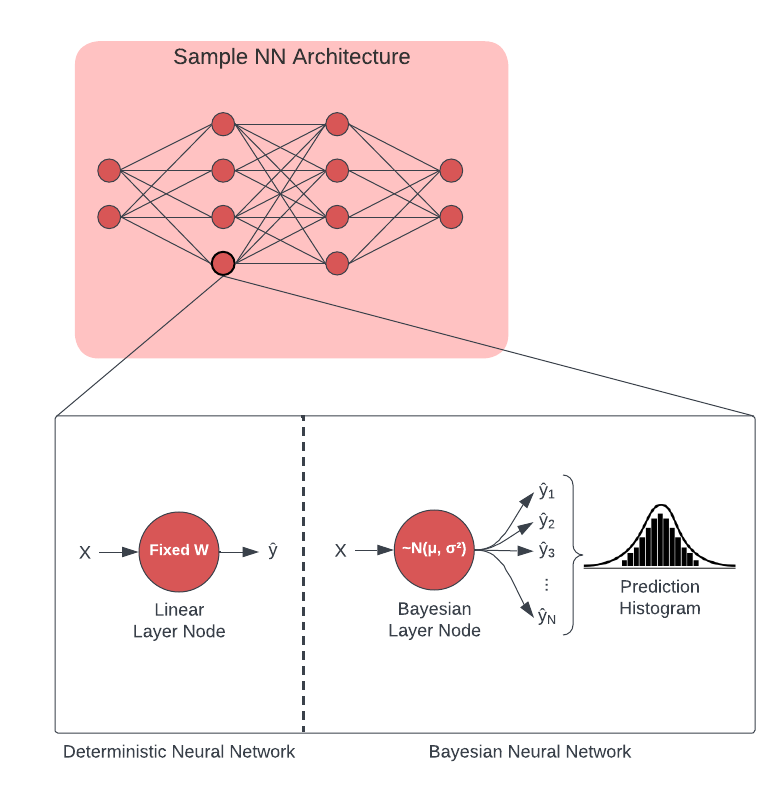
\includegraphics[width=0.85\textwidth]{bayesian_transformation.png}
    \caption{Deterministic versus Bayesian neural network architectures. Deterministic networks use fixed weights $W$ to produce point predictions, while Bayesian networks treat weights as distributions $\mathcal{N}(\mu, \sigma^2)$, generating prediction histograms through multiple stochastic forward passes to quantify epistemic uncertainty.}
    \label{fig:bayesian_transformation}
\end{figure}

Unlike standard deterministic ML methods, Bayesian methods model distributions over predictions using Bayes' rule, allowing for the quantification of uncertainty within parameters and labels. Bayesian methods treat the model parameters as random variables with distributions. Uncertainty can also be estimated from other non-deterministic methods, including deep ensembles \citep{lakshminarayanan2017}, bootstrap modeling \citep{palmer2022}, and federated learning \citep{Hanser2023}.

% TODO: this paragraph may need to go
Epistemic uncertainty is model-driven and can be reduced by collecting either more or higher quality training data. Aleatoric is data-driven and reflects the intrinsic noise in the labels.

\section{Molecular similarity and activity cliffs}
% ---- NOTES: Molecular similarity and activity cliffs ----
% Takeaway: similarity only exists relative to a representation and a coefficient; the representation is the larger choice.
% Takeaway: activity cliffs and uninformative features break the similar property principle, and neighbour-based noise detectors inherit the break.
% Paragraph 1: the similar property principle.
% - Numbered definition: structurally similar molecules tend to have similar properties \citep{Johnson1990, vanTilborg2022}.
% - This thesis relies on it in nearest-neighbour prediction, in the Gaussian process with a Tanimoto kernel on ECFP4 \citep{Ralaivola2005, moss2020}, and in noise detectors that compare a molecule's label with its neighbours' (Chapter 6).
% - The later chapters test whether a representation supports this principle. State no result here.
% Paragraph 2: similarity depends on the measure.
% - A similarity value is fixed by two choices: the representation and the coefficient \citep{Maggiora2014}.
% - \citet{Bajusz2015} compared similarity coefficients on fingerprints. Tanimoto, Dice, Cosine and Soergel were the best, and roughly equivalent.
% - Change: "changing the similarity formula yields minimal improvement if the underlying representation is weak" claims more than Bajusz2015 found. They did not test weak representations.
% - That the representation matters more than the coefficient is this thesis's own argument, not a cited result.
% - Change: "Distance-based reasoning rely" should be "relies". "\citet{Bajusz2015} et al." prints "et al." twice, and the sentence cites Bajusz2015 a second time.
% Paragraph 3: activity cliffs.
% - Numbered definition: a pair of structurally similar molecules with a large potency difference, from a small chemical change \citep{Maggiora2006, Stumpfe2012, Dablander2023}.
% - Change: the prose defines activity cliffs twice (opening paragraph and "The sharpest failure" paragraph). Keep one.
% - There is no widely accepted definition, and each similarity measure captures only part of the chemistry \citep{vanTilborg2022}.
% - Change: drop "the benchmark used in this thesis". MoleculeACE's datasets are not thesis datasets. Cite it only for its cliff rule and cliff shares.
% - This thesis counts cliffs with a different rule. A pair is similar at ECFP4 Tanimoto of at least 0.55. The activity gap is set per dataset so that 15\% of molecules are cliffs by default.
% - No source for 0.55 yet. Stumpfe, Hu and Bajorath 2019 (ACS Omega) call the choice of threshold "largely subjective". Present 0.55 as this thesis's own choice unless a source turns up.
% - The same paper sets potency thresholds per target set: the mean plus two standard deviations of analog-pair potency differences. This is the nearest precedent for a per-dataset activity gap. Not yet in the bibliography.
% Paragraph 4: why cliffs and label noise are hard to tell apart.
% - To a detector that compares a molecule with its neighbours, a cliff looks like label noise: a real, large label gap between near-identical molecules.
% - Removing cliffs as noise removes the molecules with the most structure-activity information.
% - When the neighbours' labels are noisy too, the comparison itself is unreliable.
% Paragraph 5: high dimensionality.
% - Nearest and farthest distances become nearly equal as the number of dimensions grows \citep{Beyer1999}. \citet{Aggarwal2001} extend it to each $L_k$ norm.
% - Change: the prose credits this to Aggarwal et al. alone. Cite \citet{Beyer1999} as well.
% - Aggarwal et al.'s own finding: Manhattan (L1) is preferable to Euclidean (L2) in high dimensions, and fractional norms do better still \citep{Aggarwal2001}.
% - That uninformative features dominate the distance is this thesis's argument. Chapter 4 measures it.
% - Answer to your TODO on the bib: the entries are in refs.bib. Still to fix: Dablander2023 lists "Michael Dablander"; it should be Markus Dablander.
% ---- END NOTES ----

Distance-based reasoning rely on the assumption that the data embeddings  contain quality information. When the labels are corrupted or the important features are scarce, similarity scores over-rely on compounding false or useless information, and the assumption that similar molecules have similar properties breaks down. \citet{Bajusz2015} et al. found that while the Tanimoto coefficient can be effective with binary fingerprints, changing the similarity formula yields minimal improvement if the underlying representation is weak \citep{Bajusz2015}.
This problem is further complicated by activity cliffs (ACs), which are defined as structurally similar molecules with large property differences, often due to a subtle chemical change \citep{Stumpfe2012, Dablander2023}. These molecules, which potentially contain the most important information for model prediction, can be confused with noise. Another barrier to distance-based reasoning is persistent noise across labels. The task of trying to determine if a molecule's value matches that of its neighbors becomes a lot harder when all of the neighbors have some form of noise as well. 


% TODO: hand edit
% TODO: review, needs manual review
Much of cheminformatics rests on the similar property principle: molecules that are structurally similar tend to have similar properties \citep{Johnson1990, vanTilborg2022}. 
One of the clearest applications of this principle is the use of nearest-neighbour prediction which shows up across cheminformatics workflows and in the case of this research, in the kernels used by GPs and at the basis of many noise identification algorithms.

% TODO: review, needs manual review
The difficulty with this assumption is that similarity is defined only relative to a similarity measure, and that measure is fixed by the choice of representation and
coefficient \citep{Maggiora2014}. There is no standard definition of similarity between molecules, especially when handling different molecular embeddings in a computational setting. Two molecules that are near-identical under a substructure fingerprint may be far apart under a physicochemical descriptor vector. \citet{Maggiora2014} caution that quantified similarity can be over-interpreted in this manner. 

There are many downstream tasks which rely on the concept of similarity. The second half of this thesis relies on many such tasks, and as such focuses on identifying representations that agree with this principle. 


% TODO: review, needs manual review
The sharpest failure of the similar property principle is the activity cliff: a pair of structurally similar molecules with a large difference in potency, produced by a small
chemical change \citep{Maggiora2006, Stumpfe2012}. Activity cliffs inherit the measure-dependence of the principle they violate, and there is no widely accepted definition of one
\citep{vanTilborg2022}. The MoleculeACE benchmark used in this thesis makes the choice explicit: a pair is ``highly similar'' if it exceeds 90\% similarity under at least one of
three measures --- Tanimoto on extended connectivity fingerprints, Tanimoto on scaffold fingerprints, or a scaled Levenshtein distance on SMILES strings --- and forms a cliff if
it also differs by tenfold or more in $K_i$ or EC$_{50}$ \citep{vanTilborg2022}. The soft consensus over three measures is used precisely because each captures only part of the
underlying chemistry. Cliff compounds account for between 7\% and 52\% of a dataset across the thirty targets.

% TODO: review, needs manual review
A further difficulty is dimensionality itself. \citet{Aggarwal2001} show that as the number of dimensions grows, the distance to the nearest point and the distance to the furthest
point become increasingly similar, leaving pairwise distances progressively less discriminative. Molecular representations are routinely high-dimensional and sparse, and when a
large proportion of their dimensions carry no information relevant to the property being modelled, distances computed over them are dominated by those uninformative dimensions.


% TODO: make changes to bib

\section{Noise in molecular data}
% ---- NOTES: Noise in molecular data ----
% Takeaway: real label noise comes from many sources and is not independent, identically distributed or Gaussian.
% Takeaway: label noise is not always harmful; it can act as regularisation.
% Paragraph 2: the shape of real noise is not Gaussian.
% - Studies of noise robustness usually add independent, zero-mean Gaussian error to labels.
% - \citet{Kruger2012} rejected normality of repeat bioactivity differences and fitted a Laplace distribution.
% - \citet{Kalliokoski2013}: across 16,844 pairs of repeat pIC$_{50}$ values, the widest gaps came from annotation error, not assay imprecision.
% Paragraph 3: independence and zero mean fail too.
% - \citet{Bentz2013}: 23 laboratories, P-glycoprotein transport; 62\% of the variance in log efflux ratio lay between laboratories.
% - Censoring: \citet{Svensson2025} found censored labels in 13 of 15 industrial assays; in 8, between a quarter and two thirds of labels were censored.
% - Change: the last sentence ("In this study, we tested noise conditions...") should point to Section~\ref{sec:noise_injection} and Chapter~\ref{chap:robustness}.
% Paragraph 5: instruments and detection limits.
% - \citet{Zhang1999} defines the Z-factor, which scores an assay by its signal range and signal variation. It does not cover spectrophotometric error near detection limits or radiometric background subtraction.
% - \citet{Simeonov2008} profiled the fluorescence of more than 70,000 library samples. More than 5\% were brighter than 10 nM of 4-methylumbelliferone. Compound fluorescence caused both false positives and false negatives.
% - Change: the sentence on quenching giving false negatives for potent inhibitors does not match Simeonov2008. Rewrite to the finding above.
% - Change: "systematic bia" should be "systematic bias".
% Paragraph 7: aggregation across databases.
% - Add the current ChEMBL release paper \citep{Zdrazil2023} next to Gaulton2017.
% - Change: "between 10 and 20 reported values... two orders of magnitude" is not what \citet{Kramer2012} reports. Its ChEMBL Ki pairs: mean error 0.44 pKi units, standard deviation 0.54, median 0.34. The best possible R$^2$ on large datasets is 0.81.
% - Kramer2012 also found that 90\% of repeat pairs were one measurement cited twice.
% - \citet{landrum2024}, IC$_{50}$ pairs with minimal curation: 65\% differ by more than 0.3 log units, 27\% by more than one log unit, Kendall's $\tau$ 0.51.
% - With metadata matched: 48\% differ by more than 0.3 log units, 13\% by more than one log unit, $\tau$ 0.71. Ki assays showed similar noise.
% Paragraph 8: federated learning.
% - \citet{Hanser2025} describe federated learning in drug discovery by knowledge distillation, the teacher-student set-up of Effiris.
% - Noisy and differing clients are a known problem in federated learning \citep{Fang2022}.
% - Change: "presents" should be "present"; "confidental" should be "confidential".
% Paragraph 9: annotation and structure errors.
% - Structure-curation workflow \citep{Fourches2010}.
% - Change: the prose says 1-5\% structure errors. \citet{Young2008} found 0.1\% to 3.4\% across six databases. The paper does not break errors down into SMILES parsing, tautomers or transcription, so drop that list or cite another source.
% - In their octanol/water partition case study, a misplaced Cl atom changed predictions markedly \citep{Young2008}.
% - Example from benchmark data \citep{Walters2023}: 71\% of BACE molecules have at least one undefined stereocentre. The blood-brain barrier set has 59 duplicate structures, 10 of them with conflicting labels.
% - Protonation states and counterions: point to Chapter 4, where molecules the representation cannot tell apart are counted.
% Paragraph 10: real noise is not i.i.d. or symmetric.
% - Survey of label-noise sources and consequences: \citet{Frenay2014}.
% - One sentence before the Heid2023 sentence: \citet{Kolmar2021} modelled experimental noise as Gaussian, arguing from the central limit theorem. Models that learn the trend can predict more accurately than their own training labels.
% - \citet{Heid2023} showed noise can depend on structure: nitrogen-containing functional groups carried systematic measurement deviations.
% - Chapter 6 also measures noise on real labels: repeat measurements, disagreement between laboratories, curator flags.
% Paragraph 11: label noise can regularise.
% - Change: "noise analysis and mitigation literature" should be "the label-noise literature, including learning with noisy labels". Noise mitigation is one subset of LNL.
% ---- END NOTES ----

% TODO: review, needs manual review
Real-world cheminformatics datasets contain label noise arising from multiple sources across the drug discovery pipeline. To properly model experimental noise, we must first understand where the noise is coming from.

Studies involving noise, and specifically the quantification of noise robustness, typically approach label noise by adding independent, zero-mean, Gaussian error to the labels. However, there's evidence to suggest that noise from experimental assays takes on different forms. \cite{Kruger2012} rejected normality of bioactivity differences by Anderson-Darling test and fitted a Laplace distribution instead. \citet{Kalliokoski2013} examined the widest disagreements among 16,844 pairs of repeat pIC$_{50}$ measurements and found that in almost all cases, the wide gap between repeat values was due to annotation error rather than to an imprecise assay.

Beyond just the shape, the assumptions of independence and zero mean may fail as well. \citet{Bentz2013} examined P-glycoprotein transport measurements across 23 laboratories and found that $62\%$ of the variance in log efflux ratio was due to differences between laboratories. When you pool data from different sources, each source has the potential to carry a shared offset. These sources usually contain families of related compounds, breaking the independence assumption. The zero-mean assumption is not assured either, especially when true values fall above or below an assay's detection limit, called censoring. \citet{Svensson2025} count censored labels in fifteen industrial assays, of which thirteen carry censored labels and eight sit between a quarter and two thirds censored. In this study, we tested noise conditions that vary the shape, the correlation, and the bias of injected error separately at a matched quantity.  

Assay-related variability represents a primary source of label noise in bioactivity data. High-throughput screening assays are often laden with errors from physical phenomena such as edge effects, where compounds in wells exhibit different activities at plate boundaries due to evaporation or temperature gradients \citep{Macarron2011}. Other examples include compound carryover between wells, incomplete liquid transfers, and air bubbles  \citep{Inglese2006}.  Detection reagents or unstable compounds can degrade over time, which leads to drift within a single plate run. This turns into heteroscedastic noise correlated with plate position or read time \citep{Brideau2003}.

Instrument calibration and detection limits can impact measurement accuracy. Spectrophotometric assays near detection limits exhibit higher relative error, such that signal-to-noise ratios degrade for weak binders \citep{Zhang1999}. Fluorescence quenching by test compounds introduces a systematic bia in fluorescence-based assays, resulting in false negatives for potent inhibitors that accidentally get absorbed at emission wavelengths \citep{Simeonov2008}. Radiometric assays require background subtraction and decay corrections that accumulate error, particularly for low-activity compounds where the signal barely exceeds background \citep{Zhang1999}.

Another source of noise is biological variability. Even minor variations in cell culture conditions such as seeding density, plating efficiency, growth rate, and cell cycle distribution have the potential to affect downstream tasks such as cell metabolism and drug responsiveness. Even serum properties may introduce variability \citep{Hatzis2014}. The speed of cell culture passages is even found to be a significant factor in behavior \citep{Postnikova2018}. 

Data aggregation across multiple sources compounds these individual error sources. Common databases like ChEMBL, BindingDB, and PubChem aggregate measurements from hundreds of laboratories using a diverse set of protocols, compound purities, and quality control standards \citep{Gaulton2017, Gilson2016}. The $K_i$ or IC$_{50}$ values from the same compound-target pair with between 10 and 20 reported values, often end up spanning two orders of magnitude apart, making it challenging to identify the underlying ground truth \citep{Kramer2012}. All the sources of error mentioned above regarding inconsistent experimental protocols cannot be distinguished easily from the genuine underlying value without extensive, and often unrealistic amounts of metadata \citep{Fourches2016}.


Federated datasets, a method of data aggregation centered around privacy protection, presents a particularly challenging situation for noise. In pharmaceutical research and beyond, companies often want to merge collective information without exposing proprietary data to competitors. One example of such platforms is Lhasa Limited's federated learning platform Effiris. Teacher models are first trained separately on confidental data, and then used to label a shared public chemical data set. Those results are consolidated into a federated student model \citep{Bassani2023}. While this is an effective approach of protecting intellectual property, it introduces additional label noise through the prediction errors of all the teacher models. There also exists aleatoric uncertainty from the underlying experimental measurements, many of which likely come from differing protocols, resulting in compounding label noise. 

Beyond the experimental setups, annotation errors in the data itself can arise from mis-registered structures, incorrect stereochemistry assignments, and salt form ambiguity \citep{Williams2017}. Public databases are estimated to contain 1-5\% structure errors from incorrect SMILES parsing, tautomer misassignment, or manual transcription mistakes during data entry \citep{Young2008}. Ambiguous protonation states and counterions create representation-level noise where chemically distinct samples are classified as the same \citep{Bento2020}.

These noise sources can interact with each other and present in more ways than a simple Gaussian. Unlike artificial noise injection, real-world noise is neither independent, identically distributed, nor symmetric  \citep{Heid2023}. I wanted to address this complexity in my research by examining a variety of ways of both modeling and adding noise to data sets. 

Although the general assumption in many of the noise analysis and mitigation literature is that noise, specifically label noise, will have a negative effect on the model, this is not necessarily the case. There are multiple instances of using noise as a method of regularization. Although not the optimal approach to counteracting overfitting in linear regression, adding artificial noise to labels is considered a form of regularization \citep{Ullah2024}. Furthermore, adding artificial noise drawn from a Gaussian distribution to the activation layers of a neural network is considered another form of regularization \citep{Camuto2021}. These studies indicate that the presence of noise may act as a form of regularization in some contexts. It is important to address this potential of regularization from label noise in QSAR and QSPR models.

\subsection{Artificial noise injection}\label{sec:noise_injection}
% ---- NOTES: Artificial noise injection ----
% Takeaway: the seven conditions deliver the same expected amount of noise, so a difference between conditions is a difference in pattern, not amount.
% Takeaway: each parameter comes from a published measurement error where one exists.
% Paragraph 1: what gets noise.
% - Training and validation labels get noise; test labels stay clean.
% - Change: the first sentence says validation data stay free of noise; the next says they are noised. Drop "validation and" from the first.
% Paragraph 2: the seven conditions.
% - Change: use "grouped-shifted" throughout. Paragraph 2 writes "Group shifted".
% - Change: "on specific subset" should be "on a specific subset"; "every label extends past" should be "every label that extends past".
% Paragraph 5: the parameters and where each comes from.
% - Scaffold families are taken in random order. A family is skipped if adding it would move the share of affected molecules further from 20\% than leaving it out. So the share is near 20\%, not exactly 20\%.
% - Validation draws its own families by the same rule. Under a scaffold split, validation shares no scaffold family with training.
% - Change: "62\% of the variance in Caco-2 across 23 laboratories" does not match Bentz2013. Only 11 of the 23 laboratories used Caco-2 cells.
% - The 62\% is the laboratory share of variance in log efflux ratio (digoxin, no inhibitor), cell-line data only, Bentz2013 Table 7. Cite Table 7, and word it as in "Noise in molecular data".
% - Answer to your TODO on the 20\%: no published estimate exists of how large a share of a dataset a difference between laboratories affects. So 20\% of molecules was chosen, not sourced. Whole scaffold families are drawn until about 20\% of the split is covered.
% - Censoring has no parameter here: its level is the fraction of labels clipped.
% ---- END NOTES ----

Our objective is to evaluate the robustness of QSAR models against label noise. To do so, we ``inject'' artificial noise into the labels during training while validation and test data remain free of noise. Validation labels are given noise of the same type and quantity as the training labels, drawn independently. This artificial noise simulates real-world experimental noise. The clean target label $y_i$ is replaced by a noisy label $\tilde{y}_i = y_i + \epsilon_i$, where $\epsilon_i$ is the artificial noise injected at the index $i$, the value of which is determined by a specified noise strategy. As we increased the quantity of noise, we measured how much predictive performance fell. 

We explored seven methodologies of adding noise, referred to as noise conditions (Figure~\ref{fig:noise_conditions}). Three vary the shape of the distribution from which the error is drawn. These shapes include Gaussian, Student-$t$ with $\nu = 5$, and Laplace distributions. Two conditions concentrate error on specific subset of molecules; outlier isolates a random tenth of them and grouped-wider concentrates on Bemis--Murcko scaffold families. Group shifted also applies noise to scaffolds, but instead gives each scaffold its own offset rather than a wider error. The seventh, censoring, sets a limit such that every label extends past that limit is reassigned to the limit itself. 

For a given label, every condition except censoring delivers the same expected quantity of noise at a set noise level. These levels are defined as a fraction of the standard deviation of clean training labels. The noise added to the label of molecule $i$ is
\begin{equation}
\epsilon_i = \frac{\tau}{G}\,s_i z_i,
\qquad
G = \sqrt{\frac{1}{n}\sum_{j=1}^{n} s_j^{2}}\;\;\sigma_z,
\label{eq:dose_matching}
\end{equation}
% TODO: review, needs manual review
Here $\tau$ is the target standard deviation of the noise, in the units of the label, and $z_i$ is
drawn from the condition's distribution at unit scale. The multiplier $s_i$ is $1$ for most
molecules and $\lambda = 3$ for those the condition affects, which are a random $10\%$ of molecules
under outlier and whole scaffold families covering $20\%$ of the split under grouped-wider. The
constant $\sigma_z$ is the standard deviation of $z$, equal to $1$ for the Gaussian,
$\sqrt{\nu/(\nu-2)}$ for the Student-$t$ and $\sqrt{2}$ for the Laplace. The factor $G$ divides both
of these out, so that $\epsilon$ has standard deviation $\tau$ in expectation whatever the
distribution and whichever molecules are affected.

% TODO: review, needs manual review
Grouped-shifted widens no molecule's error, and instead gives every scaffold family $g$ an offset of
its own,
\begin{equation}
\epsilon_i = \frac{\tau}{G}\left(\sqrt{\rho}\,b_{g(i)} + \sqrt{1-\rho}\,w_i\right),
\label{eq:grouped_shifted}
\end{equation}
with one draw $b$ per family and one draw $w$ per molecule. The two variances sum to $\tau^{2}$, and
the family offset carries a share $\rho$ of that total.

% TODO: No published figure exists for the fraction of scaffold families a difference between laboratories would cover, so we chose the $20\%$ above rather than sourcing it. - need to rephrase this 
We selected parameters from published measurement errors, wherever possible. As inter-laboratory error is estimated to be approximately three times intra-laboratory error, we set $\lambda = 3$ \citep{Avdeef2019}. \cite{Hampel2001} reports that $1-10\%$ of routine scientific data contains gross errors; we selected the upper bound of $10\%$. Laboratory identity accounts for $62\%$ of the variance in Caco-2 across 23 laboratories, prompting us to set $\rho = 0.62$ \citep{Bentz2013}. We took the Student-$t$ and Laplace shapes from the distributions fitted to repeated public bioactivity measurements \citep{Kruger2012}, and contaminated a fraction of the samples with a wider error according to Huber's contamination model \citep{huber1964robust}. As we found no published estimate of how large a share of a given dataset inter-laboratory differences affect, we chose to randomly select scaffolds until $20\%$ of the molecules had been covered. 

% TODO: review, needs manual review (caption)
\begin{figure}[htbp]
\centering
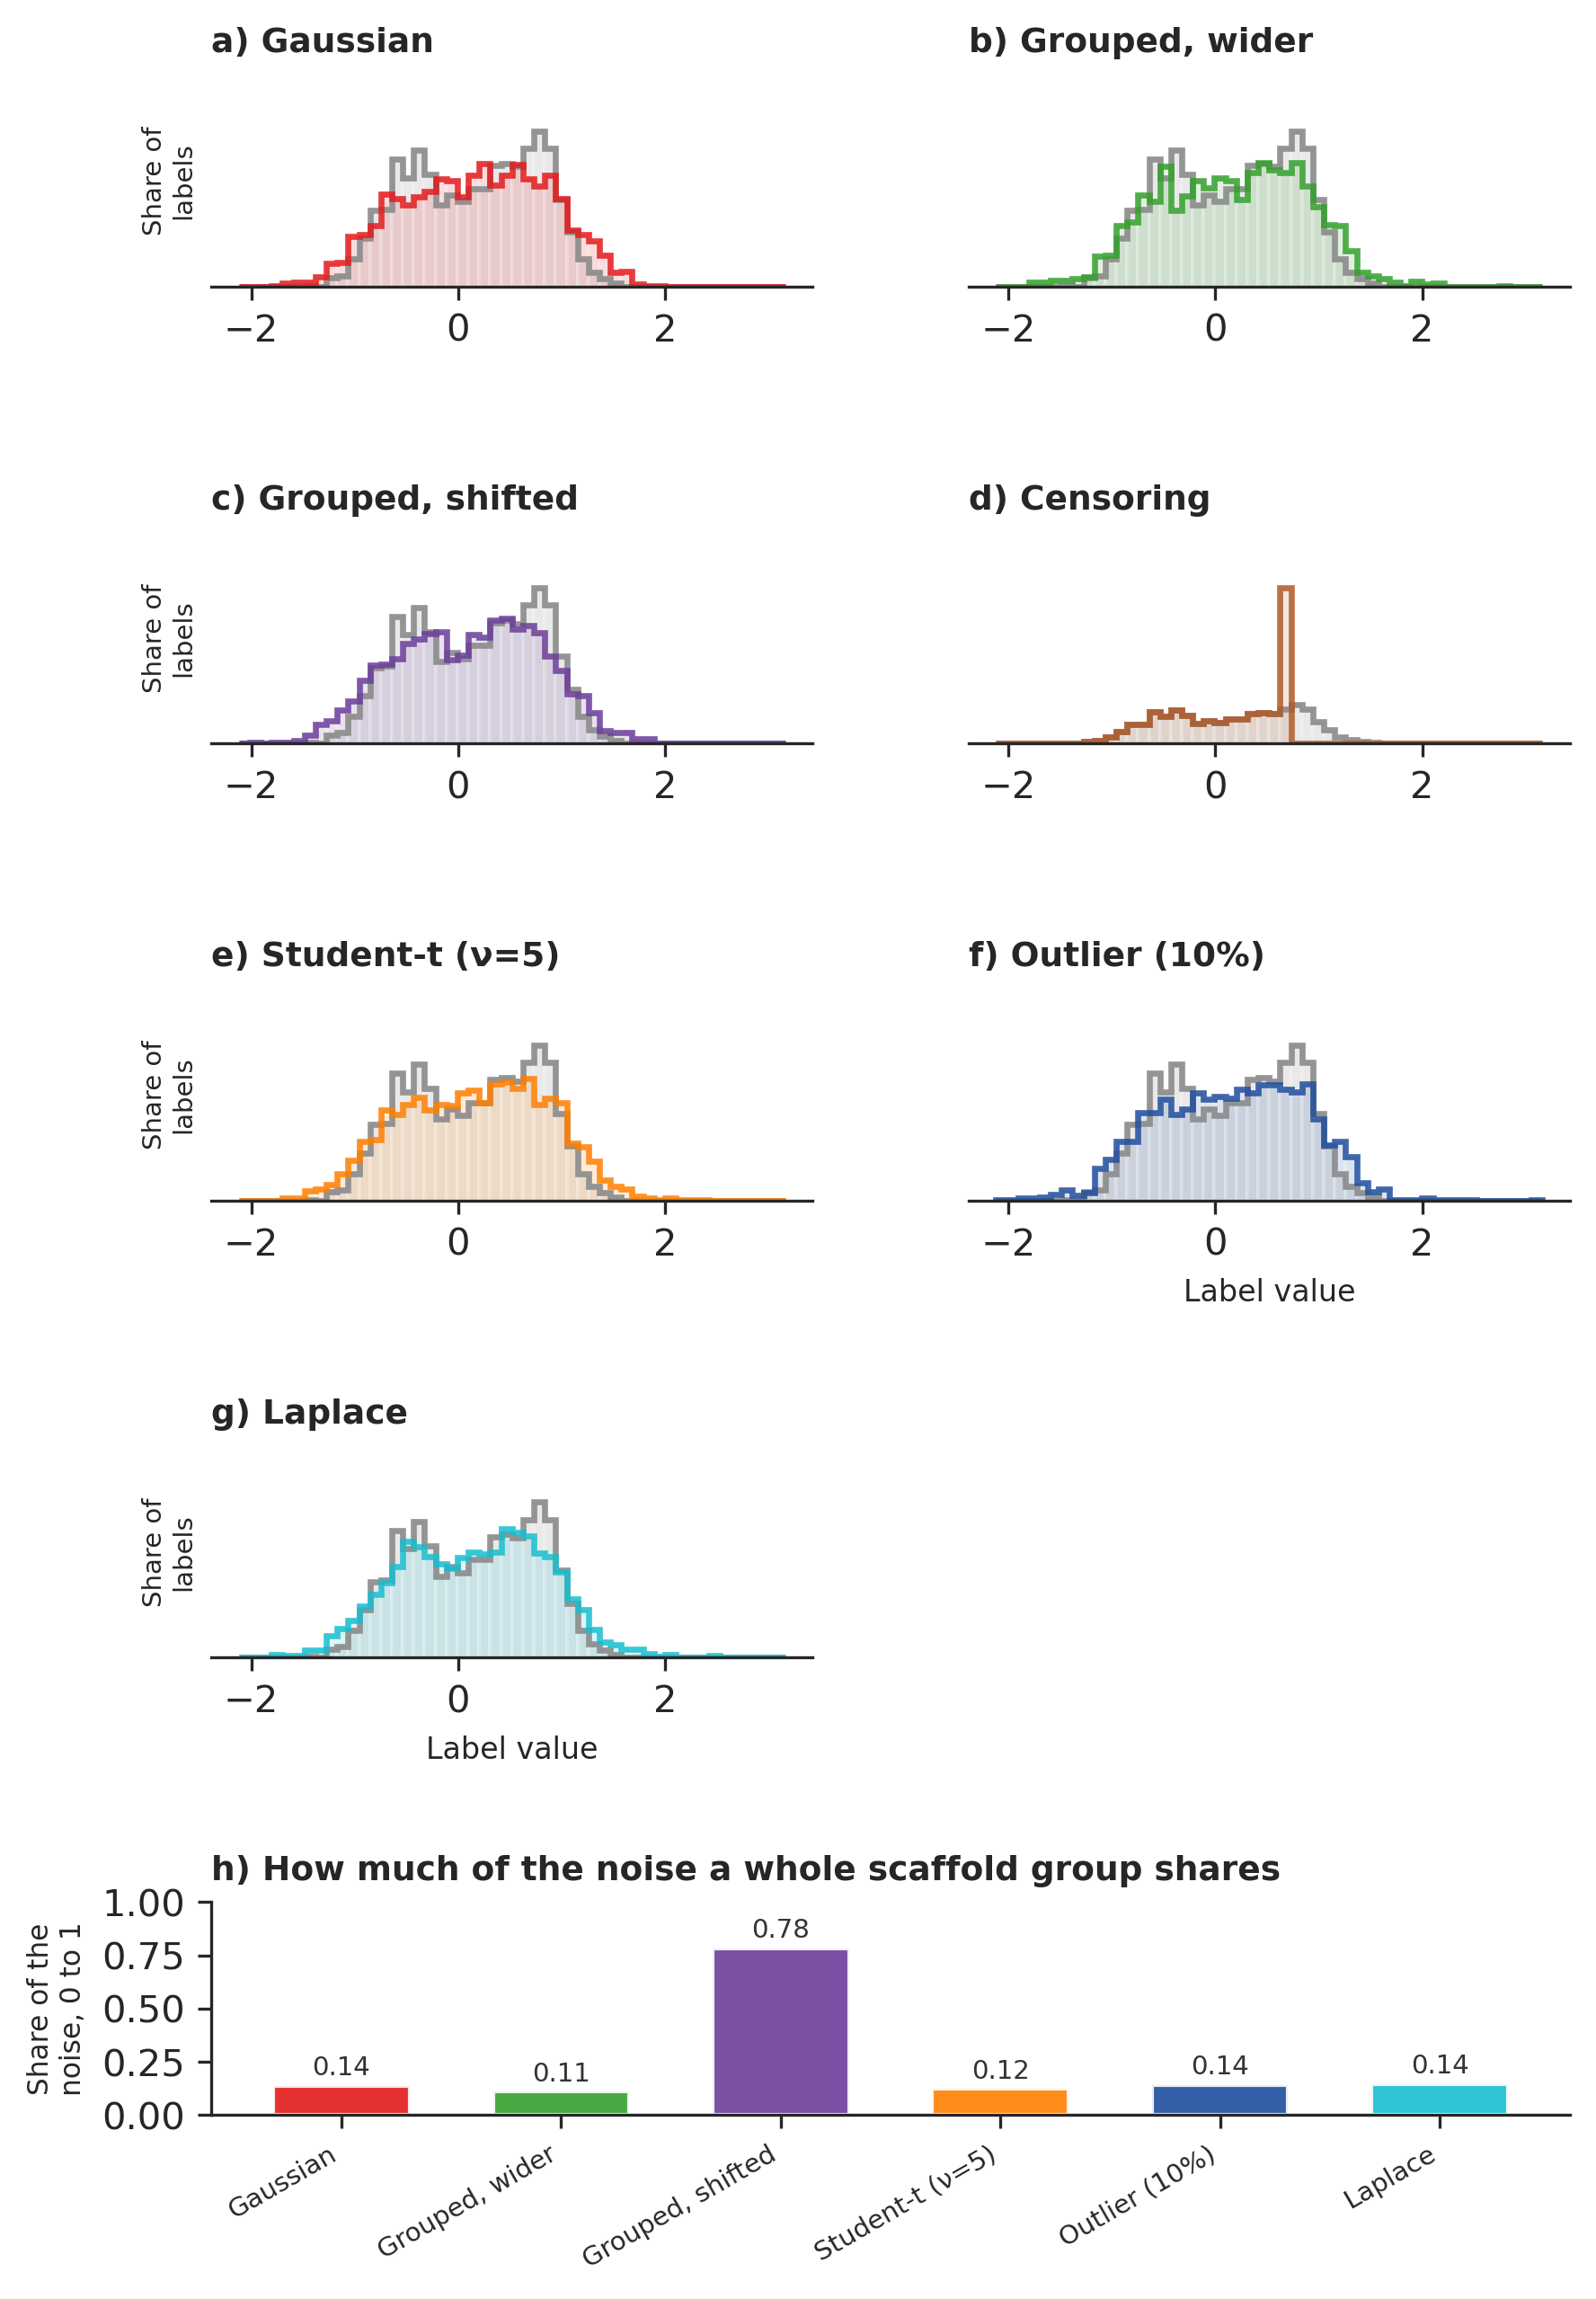
\includegraphics[width=\textwidth]{F1_noise_conditions.png}
\caption{The seven noise conditions applied to one set of labels. The labels are 2,000 synthetic
values rather than a study dataset, split at random into 40 groups that stand in for scaffold
families. a)--g) Clean labels in gray and noised labels in color, at a noise level of 0.5 of the
clean label spread. Censoring is drawn with 25\% of labels clipped, since its level is the fraction
clipped. The bottom axis is the label value and the side axis is the share of labels in each bin.
h) For each condition except censoring, the standard deviation of the mean error within a group,
divided by the standard deviation of all errors. A value near 1 means a group's labels move
together. With about 50 labels per group, noise that ignores the groups gives about 0.14.}
\label{fig:noise_conditions}
\end{figure}

% ---- NOTES: Learning with noisy labels (planned section, no heading yet) ----
% Takeaway: LNL covers every method for training a model when some labels are wrong. Noise mitigation is the subset that changes the labels before training.
% Takeaway: no single method wins, and methods that compare a molecule with its neighbours fail where similarity fails.
% Paragraph 1: what LNL is.
% - Noise mitigation changes, drops or reweights the training labels once, before a model is trained. Any model can then be fitted to the result. Examples: removal, down-weighting, smoothing, relabelling, correction.
% - Noise-robust training leaves the labels and changes how the model trains. Examples: robust losses, noise-modelling layers, regularisation, and reweighting inside the training loop (co-teaching, Meta-Weight-Net).
% - A sample-selection step taken out of its training loop and used only to delete molecules before a refit counts as noise mitigation.
% - Noise detection and noise estimation find or size noisy labels. They feed noise mitigation but are not LNL methods themselves.
% - Taxonomy of 62 deep-learning methods in five groups: robust architecture, robust regularisation, robust loss function, loss adjustment, sample selection \citep{Song2022}.
% Paragraph 2: why no single method wins.
% - No free lunch: averaged over all problems, no learning algorithm beats another \citep{Wolpert1996, Wolpert1997}.
% - Chemistry analogue: twelve algorithms on twelve bioactivity datasets with simulated experimental errors \citep{Cortes2015}.
% - Neighbour-based cleaning goes back to editing a training set by its nearest neighbours \citep{Wilson1972}. It relies on similar molecules having similar labels, which activity cliffs break.
% - QSAR models frequently fail to predict activity cliffs \citep{Dablander2023}.
% - Chapter 6 tests this.
% ---- END NOTES ----

\section{NoiseInject: a benchmarking framework}
% ---- NOTES: NoiseInject: a benchmarking framework ----
% Takeaway: NoiseInject is introduced here, before Chapters 3 and 6, because both use it.
% Paragraph 1: which work uses which noise implementation.
% - NoiseInject 1.0.0 is an open-source Python package, MIT licence \citep{noiseinject}.
% - Change: add that the label-noise experiments on the hybrid in Chapter 6 use it too.
% - QM9 is the exception: its noise comes from a separate Rust implementation of the same seven conditions. Point to Chapter 3 for that pipeline.
% - Change: the cross-check compares more than the paragraph lists. It also compares the share of labels moved by more than three times the target noise, the share of the squared error carried by the worst 5\% of labels, and the censoring limit.
% - For every condition except censoring, it also checks that the solved scale times G equals the requested noise exactly.
% ---- END NOTES ----

% TODO: review, needs manual review
The noise conditions described above are implemented twice. The three experimental datasets and
every uncertainty result use NoiseInject, an open-source Python package. QM9 uses a separate
Python--Rust precompute pipeline, which carries its own Rust implementation of the same conditions.
An executable cross-check compares the two implementations before any cluster run. Rust's and
NumPy's random number generators produce different streams, so the check compares statistics rather
than individual draws: on the same labels, groups and seeds, it compares the delivered noise, the
unit dose $G$, the median error, the number of badly corrupted labels and the number of molecules
affected.

\subsection{NoiseInject}
% ---- NOTES: NoiseInject ----
% Takeaway: the package injects each noise condition at a matched amount and reports how much performance and uncertainty quality survive.
% - Change: "In the KIRBy experiments" should be "In the experiments with the hybrid". KIRBy names only the repository.
% - Classification: Chapter 6 states its levels as the fraction of training labels flipped to the wrong class (0 to 0.40). That fraction is the target the binary search hits, on the training labels only.
% - One clause can point forward to "Noise conditions" in Chapter 6 for the flip levels.
% ---- END NOTES ----

% TODO: review, needs manual review
NoiseInject (version 1.0.0) evaluates model robustness and uncertainty calibration under artificial
label noise, for both regression and classification. It operates on label arrays and on the
predictions of any externally trained model, so it is model-agnostic. The core package depends only
on NumPy, pandas, SciPy and scikit-learn. Results are returned as \texttt{pandas} DataFrames, one
row per noise level and one aggregate summary row. The software is available under an MIT license
and archived on Zenodo \citep{noiseinject}.

% TODO: review, needs manual review
\paragraph{Regression noise.} The regression injector takes a noise shape (Gaussian, Student-$t$ or
Laplace) and a targeting rule (uniform, grouped-wider, grouped-shifted, outlier or censoring)
separately. Each named condition in the package's registry is one combination of the two with its
parameters, and the same name is written on every results row. The registry holds more settings
than this study runs: Student-$t$ at $\nu \in \{3, 5, 10\}$, and outlier contamination at $1\%$,
$5\%$ and $10\%$. It also holds an outlier variant in which the unselected molecules receive no
noise at all, rather than the base-scale noise of Equation~\ref{eq:dose_matching}.

% TODO: review, needs manual review
The requested level is the root-mean-square noise to deliver, $\tau$, in the label's own units. The
injector computes the per-molecule multipliers $s_i$ and solves for the scale $\tau / G$ in closed
form (Equation~\ref{eq:dose_matching}); there is no calibration search. A level of zero returns the
labels exactly unchanged. Which molecules are affected is drawn from a second random generator,
seeded separately from the noise draws and re-seeded on every call. The affected molecules are
therefore the same at every noise level, including zero, while the draws themselves change. Under
grouped-wider, whole scaffold families are added in random order until the fraction of affected
molecules is as close as possible to the target of $20\%$, because a fixed fraction of families
gives a very different fraction of molecules when family sizes are uneven.

% TODO: review, needs manual review
Censoring is parameterised by the fraction $f$ of labels clipped. The limit is the $(1-f)$ quantile
of the reference labels, which are the clean training labels. On the training split, the censored
set is exactly the $k = \mathrm{round}(fn)$ largest labels. On any other split it is whichever
molecules lie past the training limit.

% TODO: review, needs manual review
Each injection returns its provenance alongside the noisy labels: the target dose, the unit dose
$G$, the solved scale, the delivered root-mean-square noise (in label units and as a fraction of the
clean label standard deviation), the mean of $\epsilon$, the fraction of molecules affected, the
number and largest share of groups, and the seeds. The injector also checks the delivered amount.
The delivered dose is an estimate from a finite sample, so it is compared against a band of three
standard errors,
\begin{equation}
\left|\frac{\hat{\tau}}{\tau} - 1\right| \le \max\!\left(3\sqrt{\frac{\kappa - 1}{4\,n_{\mathrm{eff}}}},\; 0.005\right),
\qquad
n_{\mathrm{eff}} = \frac{\left(\sum_i s_i^2\right)^2}{\sum_i s_i^4},
\label{eq:dose_tolerance}
\end{equation}
where $\hat{\tau}$ is the delivered root-mean-square noise and $\kappa$ is the sample kurtosis of the
unscaled draws $z$, bounded between 3 and 60. The effective count $n_{\mathrm{eff}}$ is the number of
independent contributions the delivered dose averages over. It falls below $n$ when the noise is
concentrated on a few molecules. Under grouped-shifted it is
$n_{\mathrm{eff}} = \left(\rho^2/g_{\mathrm{eff}} + (1-\rho)^2/n\right)^{-1}$, with
$g_{\mathrm{eff}} = \left(\sum_g n_g\right)^2 / \sum_g n_g^2$ for family sizes $n_g$. At
$\nu \le 4$ the Student-$t$ has no fourth moment, so the standard error is instead
$1.3\,n_{\mathrm{eff}}^{\,2/\nu - 1}$, with the constant calibrated on the measured spread. A draw
outside the band raises a warning rather than an error. At three standard errors a correct injector
falls outside the band on about $1\%$ of draws, and the delivered amount is recorded on the row
either way.

% TODO: review, needs manual review
A second method returns the scale each molecule's region would receive without drawing any noise.
We use it to score held-out molecules against the pattern the training labels were exposed to. For
uniform and grouped-shifted noise this scale is the same for every molecule, so the package flags it
as degenerate. A rank correlation against a constant is undefined, and must not be reported as zero.

% TODO: review, needs manual review
A separate injector sizes noise against a unit the caller supplies rather than the label standard
deviation. In the KIRBy experiments the unit is the standard deviation of a model's out-of-fold residual on
the clean training labels, so the noise is sized against the error the model already makes. Its
conditions add Gaussian noise with variance equal to the level times the unit squared; move $2\%$,
$5\%$ or $10\%$ of labels by the level times the unit, with a random sign or always upwards; or add
Gaussian noise whose standard deviation follows either a per-molecule covariate or a hidden
log-normal draw. Both of the last two are scaled to the same mean variance as the first.

% TODO: review, needs manual review
\paragraph{Classification noise.} Six label-flipping strategies are provided: uniform flips; flip
rates set by class frequency; asymmetric flip rates for binary tasks; a random per-sample flip rate;
a separate flip rate for each class; and flips directed by a confusion matrix. Because the realised
flip rate differs from the nominal flip probability under most of these strategies, a binary search
finds the flip probability that produces a target fraction of changed labels.

% TODO: review, needs manual review
\paragraph{Robustness metrics.} For regression the package computes $R^2$, RMSE and mean absolute
error at every noise level. For classification it computes accuracy, and precision, recall and F1
score, both macro- and weighted-averaged, with a per-class breakdown. Robustness is read off the
retention curve $\mathrm{ret}(x) = m(x)/m(0)$, where $m$ is a bounded, higher-is-better metric
($R^2$ for regression; accuracy, F1, precision or recall for classification) and $x$ is the noise
level. The primary summary is the normalised area under that curve,
\begin{equation}
\mathrm{AUC}_{\mathrm{norm}} = \frac{1}{x_{\max} - x_{\min}} \int_{x_{\min}}^{x_{\max}} \mathrm{ret}(x)\,\mathrm{d}x,
\label{eq:auc_norm}
\end{equation}
evaluated by the trapezoid rule. It is the mean fraction of clean performance retained across the
sweep, lies near $[0, 1]$, and does not depend on how good the model was on clean labels. A
secondary summary fits $\mathrm{ret}(x) \approx \exp\!\left(-(x/\tau_W)^{\beta}\right)$. The shape
$\beta$ separates curves that hold and then collapse ($\beta > 1$) from curves that fall early and
then plateau ($\beta < 1$), and $\tau_W$ sets the scale of the decay. The fit needs at least four
noise levels. These two summaries replace the linear slope of performance against noise used in
earlier versions, which misdescribed a nonlinear curve and was coupled to clean performance. The
package also reports the clean baseline and the retention at the highest level. A flag marks any
curve that falls below zero retention, and an optional threshold withholds the curve summaries for
models whose clean baseline is too low to degrade meaningfully.

% TODO: review, needs manual review
\paragraph{Uncertainty metrics.} For a model that returns a per-sample predicted standard deviation
$u_i$, the package computes, at each noise level: the Spearman correlation between $u_i$ and the
absolute error $|y_i - \hat{y}_i|$; the empirical coverage $\frac{1}{n}\sum_i \mathbb{1}\left[|y_i -
\hat{y}_i| \le k u_i\right]$ at $k = 1$ and $k = 2$, against Gaussian targets of $68.3\%$ and
$95.4\%$; the mean interval width $\frac{1}{n}\sum_i 2u_i$; and the expected calibration error,
\begin{equation}
\mathrm{ECE} = \sum_{b=1}^{10} \frac{|B_b|}{n}\,\left|\bar{u}_b - \overline{|y - \hat{y}|}_b\right|,
\label{eq:ece}
\end{equation}
over ten equal-count bins $B_b$ of $u$. These are computed on the clean test labels. The Spearman
correlation between $u_i$ and the injected noise $|\epsilon_i|$ can only be computed where the noise
is known, which is the corrupted molecules, so it takes a separate pair of inputs. It is reported
within each noise level. A pooled correlation across all levels is also returned, under a separate
name. The pooled value mostly reflects that uncertainty and noise both rise with the level, so it
does not measure whether a model can pick out which molecules are corrupted.

% TODO: review, needs manual review
Three optional wrappers produce $u_i$ from a point predictor: split-conformal prediction for any
scikit-learn-compatible model, optionally scaled by the label spread of each molecule's nearest
training neighbours; an exact Gaussian process with a Tanimoto or RBF kernel, via \texttt{Gauche}
\citep{gauche}; and Monte Carlo dropout for any \texttt{PyTorch} network \citep{gal2016}. Example
notebooks and scripts cover regression and classification end to end.


\section{Evaluation methodology}

% ---- NOTES: Evaluation methodology ----
% Takeaway: every split and every fold in the thesis is group-aware; no random split is used anywhere.
% Takeaway: the metric families are named once here; each chapter says which one it uses.
% Paragraph 1 (new, before the metrics): why never at random.
% - All members of a group land on the same side of every split and fold.
% - A random split puts close structural analogues on both sides. The score then rewards recall of near-copies, not prediction \citep{Wallach2018, Yang2019}.
% - The same problem exists for sequence data: shared positions across splits let a model memorise site effects \citep{Notin2023, Vieira2026}.
% Paragraph 2: the small-molecule group.
% - Group = the Bemis-Murcko scaffold: ring systems plus the linkers between them, side chains removed \citep{Bemis1996}. Computed with RDKit \citep{rdkit}.
% - Chapter 3: the scaffold ignores stereochemistry, as do its fingerprints, so stereoisomers share a group. Each distinct acyclic molecule is its own group. Groups go to the 80/10/10 splits in random order, not largest first.
% - Chapters 5 and 6 differ in three ways. The scaffold keeps any stereochemistry written in it. All acyclic molecules share one group. Regression folds place the largest groups first.
% - Do not call this "the DeepChem scaffold split". DeepChem's splitter puts all acyclic molecules into one group and fills training largest-first.
% - Optional contrast: on the first 2,000 QM9 molecules (851 acyclic, 42.5\%), DeepChem's split put 53.2\% acyclic molecules in training and 0.0\% in validation and test.
% Paragraph 3: how folds are formed.
% - Regression: group k-fold. Each group, largest first, goes to the fold holding fewest molecules so far.
% - Classification: stratified group k-fold, which keeps class balance across folds and each group inside one fold.
% - With fewer groups than folds, the number of folds drops to the number of groups. With a single group, the run stops with an error. It never falls back to a random split.
% - Chapter 3 uses ten replicate draws of QM9 (each a fresh grouped 80/10/10 split) and five grouped folds on the three assay datasets.
% - Non-molecule datasets use their own groups (antibody sequence-identity clusters, reaction additives, chromosomes, tissue source sites). Point to Chapter 5, "Datasets and splitting".
% Paragraph 4: predictive metrics.
% - Regression: RMSE and R$^2$, plus Spearman's $\rho$ where ranking matters.
% - Classification: accuracy and F1, AUROC, and MCC. Which metric each dataset uses is set in Chapter 5, "Models and metrics".
% Paragraph 5: uncertainty metrics.
% - A higher rank correlation means the uncertainty picks out the worse predictions.
% - The rank correlation with injected noise is reported within each noise level. The pooled value across levels mostly reflects that both rise with the level.
% ---- END NOTES ----

Root mean squared error (RMSE) and the coefficient of determination ($R^2$) were primarily used to compare QSAR predictive performance.


When evaluating uncertainty, we assessed the relationship between predicted uncertainty and prediction quality. Spearman's rank correlation coefficient ($\rho$) was used to quantify the relationship between predicted uncertainty ($u_i$) and absolute error ($|y_i - \hat{y}_i|$), as well as between predicted uncertainty and injected noise magnitude. Higher correlations indicate that the model's uncertainty estimates reliably identify predictions that are likely to be incorrect.

% TODO: review, needs manual review
For probabilistic models, empirical coverage at $1\sigma$ and $2\sigma$ and the expected calibration error (Equation~\ref{eq:ece}) are defined with the NoiseInject uncertainty metrics above.

\section{Conclusions}

% ---- NOTES: Conclusions ----
% Takeaway: a predictor is a representation paired with a model; Chapter 3 asks which of the two governs how badly a predictor degrades under label noise.
% Paragraph 1: 3-4 sentences.
% - Sentence 1: both halves of a predictor, the representation and the model, have now been introduced.
% - Sentence 2: real assay noise is not independent, identically distributed or symmetric. The artificial noise model has seven conditions. LNL methods have been set out, with noise mitigation as the subset that acts on the labels.
% - No single LNL method wins on every dataset.
% - Sentence 3: NoiseInject injects the conditions and reports robustness and uncertainty metrics. The evaluation section fixes the splits and metrics.
% - Sentence 4: Chapter 3 asks whether the representation or the model architecture governs how badly a predictor degrades under label noise. Point to Chapter 1 for its four questions.
% - Optional: the representations, similarity definitions and noise conditions are reused in Chapters 4 to 6.
% ---- END NOTES ----
\todo[inline, color=yellow!40]{Write the Background chapter's closing paragraph.}
